\documentclass[conference]{IEEEtran}
\IEEEoverridecommandlockouts
% The preceding line is only needed to identify funding in the first footnote. If that is unneeded, please comment it out.
%Template version as of 6/27/2024

\usepackage{cite}
\usepackage{amsmath,amssymb,amsfonts}
\usepackage{algorithmic}
\usepackage{graphicx}
\usepackage{textcomp}
\usepackage{xcolor}
\usepackage{listings}
\usepackage{fancyvrb}
\usepackage{framed}
\usepackage[listings,skins]{tcolorbox}

\def\BibTeX{{\rm B\kern-.05em{\sc i\kern-.025em b}\kern-.08em
    T\kern-.1667em\lower.7ex\hbox{E}\kern-.125emX}}
\begin{document}

\title{Conference Paper Title*\\
{\footnotesize \textsuperscript{*}Note: Sub-titles are not captured for https://ieeexplore.ieee.org  and
should not be used}
\thanks{Identify applicable funding agency here. If none, delete this.}
}

\author{\IEEEauthorblockN{1\textsuperscript{st} Given Name Surname}
\IEEEauthorblockA{\textit{dept. name of organization (of Aff.)} \\
\textit{name of organization (of Aff.)}\\
City, Country \\
email address or ORCID}
\and
\IEEEauthorblockN{2\textsuperscript{nd} Given Name Surname}
\IEEEauthorblockA{\textit{dept. name of organization (of Aff.)} \\
\textit{name of organization (of Aff.)}\\
City, Country \\
email address or ORCID}
\and
\IEEEauthorblockN{3\textsuperscript{rd} Given Name Surname}
\IEEEauthorblockA{\textit{dept. name of organization (of Aff.)} \\
\textit{name of organization (of Aff.)}\\
City, Country \\
email address or ORCID}
\and
\IEEEauthorblockN{4\textsuperscript{th} Given Name Surname}
\IEEEauthorblockA{\textit{dept. name of organization (of Aff.)} \\
\textit{name of organization (of Aff.)}\\
City, Country \\
email address or ORCID}
\and
\IEEEauthorblockN{5\textsuperscript{th} Given Name Surname}
\IEEEauthorblockA{\textit{dept. name of organization (of Aff.)} \\
\textit{name of organization (of Aff.)}\\
City, Country \\
email address or ORCID}
\and
\IEEEauthorblockN{6\textsuperscript{th} Given Name Surname}
\IEEEauthorblockA{\textit{dept. name of organization (of Aff.)} \\
\textit{name of organization (of Aff.)}\\
City, Country \\
email address or ORCID}
}

\maketitle

\begin{abstract}
This document is a model and instructions for \LaTeX.
This and the IEEEtran.cls file define the components of your paper [title, text, heads, etc.]. *CRITICAL: Do Not Use Symbols, Special Characters, Footnotes, 
or Math in Paper Title or Abstract.
\end{abstract}

\begin{IEEEkeywords}
component, formatting, style, styling, insert.
\end{IEEEkeywords}

\section{Introduction}
The manual parallel implementation of numerical algorithms for modern supercomputers is often complicated. 
This is due to the increasing complexity and heterogeneity of the supercomputers which compels a numerical parallel 
program developer to deal with system parallel programming problems such as efficient load distribution, scheduling, etc. 
Otherwise, costly computational resources are wasted.
However, this is often beyond the developer's scope. This raises the problem of the automation of the numerical 
parallel programming. In order to address this problem a variety of automated parallel programming systems, languages 
and tools have been actively developed for the recent decades. 
Of interest are the tools that allow the automated construction of a parallel program for a distributed memory 
parallel computer from a numerical algorithm description. 
The following classes of such automated tools can be considered. General purpose tools are able to automatically 
construct a parallel program from any given numerical algorithm description. The price for such versatility is 
often relatively poor performance of the automatically constructed programs. On the contrary, specialized tools can 
only handle a limited class of numerical algorithms (for example, \cite{dplasma} is designed for dense linear algebra domain). 
Despite that, such specialized automated parallel program generating tools are able to employ 
domain-specific optimizations and parallel programming techniques. This often improves the constructed parallel 
programs performance significantly. However, it is clear that the problem of the automation of the numerical 
parallel programming is still far from solved.

In this paper ParSolGen (Parallel Solvers Generator), an automated parallel programs construction 
tool, is presented. ParSolGen constructs a highly efficient parallel program from a given numerical 
algorithm description written in ParSolGen language. Unlike other general purpose and domain-specific 
tools, systems and languages, ParSolGen accumulates various domain-specific 
parallel program construction algorithms and techniques within a single tool. Instead of performing 
sophisticated information dependencies analysis of the input numerical algorithm description or 
employing a general purpose run-time system approach, ParSolGen classifies the input numerical 
algorithm description. Depending on the classification result ParSolGen selects a proper domain-specific module 
that is suitable for the parallel program construction for the determined numerical algorithms class. 
This allows leveraging the advantages of domain-specific tools with the versatility approaching 
that of general purpose tools. Also such domain-specific parallel program construction modules 
accumulation enables ParSolGen to employ well-known manual parallel programming techniques 
in the automated parallel program construction.

The rest of the paper is organized as follows. Section 2 provides related work overview.

\section{Related work}
The variety of automated parallel programming tools, languages and systems have been actively developed 
for decades. General purpose run-time systems allow the automated execution of an executive representation 
of a numerical algorithm in a distributed manner. A numerical algorithm is represented as a DAG 
(Directed Acyclic Graph) of tasks with each task being associated with a user-provided implementation (kernel). 
The DAG is fed into the input of the run-time system which 
executes it on a supercomputer. Legion \cite{legion}, Charm++ \cite{charm, charm1}, QUARK \cite{quark} and 
StarPU \cite{starpu} can serve as illustrative examples of this approach. Legion uses regions (named sets of objects) concept to express data locality 
and uses those regions to describe the organization of data and information dependencies between tasks. 
Charm++ describes a numerical algorithm as a DAG of so called chares (computational tasks). Chares can communicate 
to each other by sending and receiving asynchronous messages. QUARK and 
StarPU are both task-based runtime systems allowing the one to submit tasks through the API of run-time system. 
Both systems build tasks DAG automatically and then execute it. Such general-purpose run-time systems are 
able to handle any given DAG representation of a numerical algorithm. Despite that, the tasks DAG representation 
often is not sufficient for the further classification of a numerical algorithm. This limits the 
possibilities of the accumulation of domain-specific parallel program construction modules in such systems.

There are also domain-specific languages and tools that partially automate the development of parallel 
implementations for specific classes of numerical algorithms. Halide \cite{halide} provides a domain-specific language 
allowing expressing schedules of stages of an image processing pipeline. Helide compiler is able to 
automatically construct a parallel implementation of a given image processing pipeline description. 
DPLASMA \cite{dplasma} allows the automated execution of a DAG representation of a dense linear algebra algorithm. It 
employs domain-specific DAG execution techniques which are implemented in the underlying DAGuE \cite{dague} engine. 
Such tools are not universal and can handle only a limited numerical algorithms class. Despite that, 
such systems employ domain-specific parallel program construction techniques and optimizations which 
improve the constructed parallel programs performance.

Of interest are automated parallel programming systems that combine a general purpose compiler of 
a high-level DSL and a general run-time system. Regent \cite{regent. regent1} and LuNA \cite{luna} are the examples of such systems. 
Regent compiler optimizes the input numerical algorithm description written in Regent DSL and generates 
an executable representation of it. This executive representation of the input numerical algorithm can then 
be executed by Legion run-time system. Similarly, LuNA consists of a DSL compiler and a general purpose run-time system. LuNA compiler analyzes the input algorithm description written in LuNA language and generates an executive 
representation of the input numerical algorithm which is then executed by LuNA run-time system. The systems also provide powerful means to provide specialized support of parallel program construction and execution, because execution control algorithms are excluded from the algorithm description. Thus program construction and execution can be varied freely to support efficient execution of applied algorithms in particular subject domains. The systems are therefore suitable for accumulating various system algorithms for different subject domains. 

This work extends LuNA project by providing powerful means to provide specialized support of the automated parallel program construction \cite{luna1}.  Unlike LuNA, ParSolGen language supports additional domain-specific operators (for example, vector operators such as dot-product) and types of variables, arrays and array elements. These language extensions provide the ParSolGen compiler with more information 
about the structure of the input numerical algorithm, enabling its proper classification.

\subsection{Numerical algorithm representation}
In ParSolGen algorithm is represented as a tuple of three sets (potentially infinite): a set of operations, a set of  
variables and a set of arrays. 
Variables store arbitrary data (for example: matrix blocks, vector blocks, single values, etc.). Each variable is assigned its type and an integer (version of the variable). Two different versions of a variable 
are considered as two independent variables by ParSolGen compiler. However, the values of these two variables can 
be stored within the same memory location. Variables can be aggregated into n-dimensional arrays in a manner similar to most procedural programming languages. Each operation is associated with two sets: a set of input variables and 
a set of output variables. An operation computes the values of the input variable values from the given 
values of the output variables. This is done by executing an associated sequential subroutine (kernel) 
provided by the developer of the numerical algorithm 
(for example: vector blocks multiplication, two values sum, etc.). An operation 
can be executed when all its input variable values are computed (in particular if the set of the input variables is empty). After an operation is executed 
the values of its output variables are considered computed and thus there appear other operations which can 
be executed. The algorithm description is considered executed when all operations are executed. 
In the rest of the paper, the described numerical algorithm representation is referred to as \textit{graph representation}.

An example of graph representation of the algorithm for summing vector elements is illustrated pic. 2. For 
illustrative purposes, it is illustrated as a DAG (Directed Acyclic Graph) of operations and variables. 
The edges of the DAG represent the information dependencies.
Array \textit{A} is 1-dimensional array of vector blocks each being a regular C-style 
1-dimensional array of floating point values.
Notation \textit{A\{v\}[i]} denotes an element of 1-dimensional array \textit{A} with 
index \textit{i} and version \textit{v}.

\subsection{ParSolGen language}
ParSolGen language provides convenient means of describing graph representation of numerical algorithms.
The following main statements are supported: variable, array, subroutine and 
operation declaration statements, for and while loop statements and conditional statements.
Consider the following example of the algorithm for summing two vectors described in ParSolGen.

\begin{lstlisting}[frame=single]
import init_vec(in int i, in int blockn,
	out Array<double> vec[blockn]);
import print_vec(in int i, in int blockn,
	in Array<double> x[blockn]);
import vec_sum(in int blockn,
	in Array<double> x[blockn],
	in Array<double> x1[blockn],
	out Array<double> y[blockn]);

...

int blockn = 10;
int nb = 5;

Array<double[blockn]> a[nb];
Array<double[blockn]> b[nb];
Array<double[blockn]> c[nb];

for (int i = 0; i < nb; ++i)
{
	init_vec(i, blockn, a[i]);
	init_vec(i, blockn, b[i]);
}

for (int i = 0; i < nb; ++i)
{
	vec_sum(blockn, a[i], b[i], c[i]);
}
\end{lstlisting}

Two integer variables (\textit{i} and \textit{j}) are declared. Three declared one-dimensional arrays \textit{a}, \textit{b} and \textit{c} 
consist of \textit{nb} elements. Each element is also an one-dimensional array storing \textit{blockn} double 
precision floating point values. These three arrays can be considered as blocked vectors with each one-dimensional 
block being an element of a one-dimensional ParSolGen array. 
For-loop statement is used to describe a set of operations 
each associated with kernel \textit{init\_vec} by using \textit{import} statement. Each operation takes values of 
\textit{i} and \textit{blockn} as input and computes the value of \textit{i}-th element of array \textit{a} (or 
\textit{b} correspondingly). Similarly, the second for-statement describes a set of \textit{nb} operations, each 
associated with \textit{vec\_sum} kernel. These operations compute the values of the corresponding \textit{i}-th 
elements of array \textit{c} by given values of variable \textit{blockn} and the values of \textit{i}-th elements of
\textit{a} and \textit{b}. The implementation of the kernels is provided by the numerical algorithm developer. For 
each kernel a C++ sequential implementation is required. The graph representation corresponding to the given example 
is illustrated in fig 3.

The below code sample illustrates the description of sparse CSR matrix-vector product: \(y = A*x\), where 
\textit{x} is an input vector, \textit{A} is a CSR matrix and \textit{y} is an output vector storing the result. 
Vectors are represented as 1-dimensional arrays of vector blocks (each vector stores \textit{nb} vector blocks, each 
block is a 1-dimensional array of \textit{blockn} double precision floating point values). The input CSR matrix 
(\textit{A}) is represented as a 2-dimensional array of CSR blocks.
\begin{lstlisting}[frame=single]
//...

Array<int> ia[n+1];
Array<int> ja[nnz];
Array<double> a[nnz];

//...

BlockedCSRMatrix<double[][]> A = {n, n, 
	nnz, nb, nb, ia, ja, a};

Array<double[blockn]> x[nb];
Array<double[blockn]> y[nb];

//...

for (int i = 0; i < nb; ++i) {
	int v = 0;
	for (int j = 0; j < nb; ++j) {
		if (!%zero(A[i][j])) {
			csr_mv(nb, 
				blockn, 
				A[i][j], 
				x[j], 
				y{v}[i], 
				y{v+1}[i]);
			v = v + 1;
		}
	}
}
\end{lstlisting}
In the above example the input matrix is initialized using regular CSR arrays \textit{ia}, \textit{ja} and 
\textit{a}. Each CSR matrix block can be checked for emptiness by using \textit{\%zero} expression which is 
\textit{true} if the input CSR matrix block is empty and only stores zero values. The kernel \textit{csr\_mv} 
computes \( y[i] = y[i] + A[i][j] * x[i] \), where \textit{A[i][j]} is a CSR matrix block, 
\textit{y[i]} and \textit{x[i]} are the corresponding vector blocks. The use of two versions of each \textit{y[i]} vector 
block enables ParSolGen compiler to store the values of these formally independent vector blocks within the same 
memory location. This allows overwriting the values of \textit{y} vector reducing the potential run-time overhead 
introduced by the management of vector block instances.


\section{ParSolGen architecture}
ParSolGen consists of two main parts: a classifying compiler and a set of domain-specific run-time systems. 
ParSolGen compiler parses the input numerical algorithm description written in ParSolGen language and feeds it into 
the input of classifier. The classifier divides the input numerical algorithm description into non-intersecrting 
subsets of ParSolGen language statements according to the class to which each statement belongs. Then 
the C++ parallel program is generated for each classified statements subset using the corresponding domain-specific 
code generation module. Each domain-specific code generation module is only suitable for a certain restricted 
numerical algorithms class (for example, for sparse linear algebra or stencil based numerical algorithms). 
The generated program can be 
linked to the corresponding domain-specific run-time systems if needed (for example, if the static code generation is not possible there is a need for dynamic load balancing support).
The process is illustrated on fig. 4.


\subsection{Maintaining the Integrity of the Specifications}

The IEEEtran class file is used to format your paper and style the text. All margins, 
column widths, line spaces, and text fonts are prescribed; please do not 
alter them. You may note peculiarities. For example, the head margin
measures proportionately more than is customary. This measurement 
and others are deliberate, using specifications that anticipate your paper 
as one part of the entire proceedings, and not as an independent document. 
Please do not revise any of the current designations.

\section{Prepare Your Paper Before Styling}
Before you begin to format your paper, first write and save the content as a 
separate text file. Complete all content and organizational editing before 
formatting. Please note sections \ref{AA} to \ref{FAT} below for more information on 
proofreading, spelling and grammar.

Keep your text and graphic files separate until after the text has been 
formatted and styled. Do not number text heads---{\LaTeX} will do that 
for you.

\subsection{Abbreviations and Acronyms}\label{AA}
Define abbreviations and acronyms the first time they are used in the text, 
even after they have been defined in the abstract. Abbreviations such as 
IEEE, SI, MKS, CGS, ac, dc, and rms do not have to be defined. Do not use 
abbreviations in the title or heads unless they are unavoidable.

\subsection{Units}
\begin{itemize}
\item Use either SI (MKS) or CGS as primary units. (SI units are encouraged.) English units may be used as secondary units (in parentheses). An exception would be the use of English units as identifiers in trade, such as ``3.5-inch disk drive''.
\item Avoid combining SI and CGS units, such as current in amperes and magnetic field in oersteds. This often leads to confusion because equations do not balance dimensionally. If you must use mixed units, clearly state the units for each quantity that you use in an equation.
\item Do not mix complete spellings and abbreviations of units: ``Wb/m\textsuperscript{2}'' or ``webers per square meter'', not ``webers/m\textsuperscript{2}''. Spell out units when they appear in text: ``. . . a few henries'', not ``. . . a few H''.
\item Use a zero before decimal points: ``0.25'', not ``.25''. Use ``cm\textsuperscript{3}'', not ``cc''.)
\end{itemize}

\subsection{Equations}
Number equations consecutively. To make your 
equations more compact, you may use the solidus (~/~), the exp function, or 
appropriate exponents. Italicize Roman symbols for quantities and variables, 
but not Greek symbols. Use a long dash rather than a hyphen for a minus 
sign. Punctuate equations with commas or periods when they are part of a 
sentence, as in:
\begin{equation}
a+b=\gamma\label{eq}
\end{equation}

Be sure that the 
symbols in your equation have been defined before or immediately following 
the equation. Use ``\eqref{eq}'', not ``Eq.~\eqref{eq}'' or ``equation \eqref{eq}'', except at 
the beginning of a sentence: ``Equation \eqref{eq} is . . .''

\subsection{\LaTeX-Specific Advice}

Please use ``soft'' (e.g., \verb|\eqref{Eq}|) cross references instead
of ``hard'' references (e.g., \verb|(1)|). That will make it possible
to combine sections, add equations, or change the order of figures or
citations without having to go through the file line by line.

Please don't use the \verb|{eqnarray}| equation environment. Use
\verb|{align}| or \verb|{IEEEeqnarray}| instead. The \verb|{eqnarray}|
environment leaves unsightly spaces around relation symbols.

Please note that the \verb|{subequations}| environment in {\LaTeX}
will increment the main equation counter even when there are no
equation numbers displayed. If you forget that, you might write an
article in which the equation numbers skip from (17) to (20), causing
the copy editors to wonder if you've discovered a new method of
counting.

{\BibTeX} does not work by magic. It doesn't get the bibliographic
data from thin air but from .bib files. If you use {\BibTeX} to produce a
bibliography you must send the .bib files. 

{\LaTeX} can't read your mind. If you assign the same label to a
subsubsection and a table, you might find that Table I has been cross
referenced as Table IV-B3. 

{\LaTeX} does not have precognitive abilities. If you put a
\verb|\label| command before the command that updates the counter it's
supposed to be using, the label will pick up the last counter to be
cross referenced instead. In particular, a \verb|\label| command
should not go before the caption of a figure or a table.

Do not use \verb|\nonumber| inside the \verb|{array}| environment. It
will not stop equation numbers inside \verb|{array}| (there won't be
any anyway) and it might stop a wanted equation number in the
surrounding equation.

\subsection{Some Common Mistakes}\label{SCM}
\begin{itemize}
\item The word ``data'' is plural, not singular.
\item The subscript for the permeability of vacuum $\mu_{0}$, and other common scientific constants, is zero with subscript formatting, not a lowercase letter ``o''.
\item In American English, commas, semicolons, periods, question and exclamation marks are located within quotation marks only when a complete thought or name is cited, such as a title or full quotation. When quotation marks are used, instead of a bold or italic typeface, to highlight a word or phrase, punctuation should appear outside of the quotation marks. A parenthetical phrase or statement at the end of a sentence is punctuated outside of the closing parenthesis (like this). (A parenthetical sentence is punctuated within the parentheses.)
\item A graph within a graph is an ``inset'', not an ``insert''. The word alternatively is preferred to the word ``alternately'' (unless you really mean something that alternates).
\item Do not use the word ``essentially'' to mean ``approximately'' or ``effectively''.
\item In your paper title, if the words ``that uses'' can accurately replace the word ``using'', capitalize the ``u''; if not, keep using lower-cased.
\item Be aware of the different meanings of the homophones ``affect'' and ``effect'', ``complement'' and ``compliment'', ``discreet'' and ``discrete'', ``principal'' and ``principle''.
\item Do not confuse ``imply'' and ``infer''.
\item The prefix ``non'' is not a word; it should be joined to the word it modifies, usually without a hyphen.
\item There is no period after the ``et'' in the Latin abbreviation ``et al.''.
\item The abbreviation ``i.e.'' means ``that is'', and the abbreviation ``e.g.'' means ``for example''.
\end{itemize}
An excellent style manual for science writers is \cite{b7}.

\subsection{Authors and Affiliations}\label{AAA}
\textbf{The class file is designed for, but not limited to, six authors.} A 
minimum of one author is required for all conference articles. Author names 
should be listed starting from left to right and then moving down to the 
next line. This is the author sequence that will be used in future citations 
and by indexing services. Names should not be listed in columns nor group by 
affiliation. Please keep your affiliations as succinct as possible (for 
example, do not differentiate among departments of the same organization).

\subsection{Identify the Headings}\label{ITH}
Headings, or heads, are organizational devices that guide the reader through 
your paper. There are two types: component heads and text heads.

Component heads identify the different components of your paper and are not 
topically subordinate to each other. Examples include Acknowledgments and 
References and, for these, the correct style to use is ``Heading 5''. Use 
``figure caption'' for your Figure captions, and ``table head'' for your 
table title. Run-in heads, such as ``Abstract'', will require you to apply a 
style (in this case, italic) in addition to the style provided by the drop 
down menu to differentiate the head from the text.

Text heads organize the topics on a relational, hierarchical basis. For 
example, the paper title is the primary text head because all subsequent 
material relates and elaborates on this one topic. If there are two or more 
sub-topics, the next level head (uppercase Roman numerals) should be used 
and, conversely, if there are not at least two sub-topics, then no subheads 
should be introduced.

\subsection{Figures and Tables}\label{FAT}
\paragraph{Positioning Figures and Tables} Place figures and tables at the top and 
bottom of columns. Avoid placing them in the middle of columns. Large 
figures and tables may span across both columns. Figure captions should be 
below the figures; table heads should appear above the tables. Insert 
figures and tables after they are cited in the text. Use the abbreviation 
``Fig.~\ref{fig}'', even at the beginning of a sentence.

\begin{table}[htbp]
\caption{Table Type Styles}
\begin{center}
\begin{tabular}{|c|c|c|c|}
\hline
\textbf{Table}&\multicolumn{3}{|c|}{\textbf{Table Column Head}} \\
\cline{2-4} 
\textbf{Head} & \textbf{\textit{Table column subhead}}& \textbf{\textit{Subhead}}& \textbf{\textit{Subhead}} \\
\hline
copy& More table copy$^{\mathrm{a}}$& &  \\
\hline
\multicolumn{4}{l}{$^{\mathrm{a}}$Sample of a Table footnote.}
\end{tabular}
\label{tab1}
\end{center}
\end{table}

\begin{figure}[htbp]
\centerline{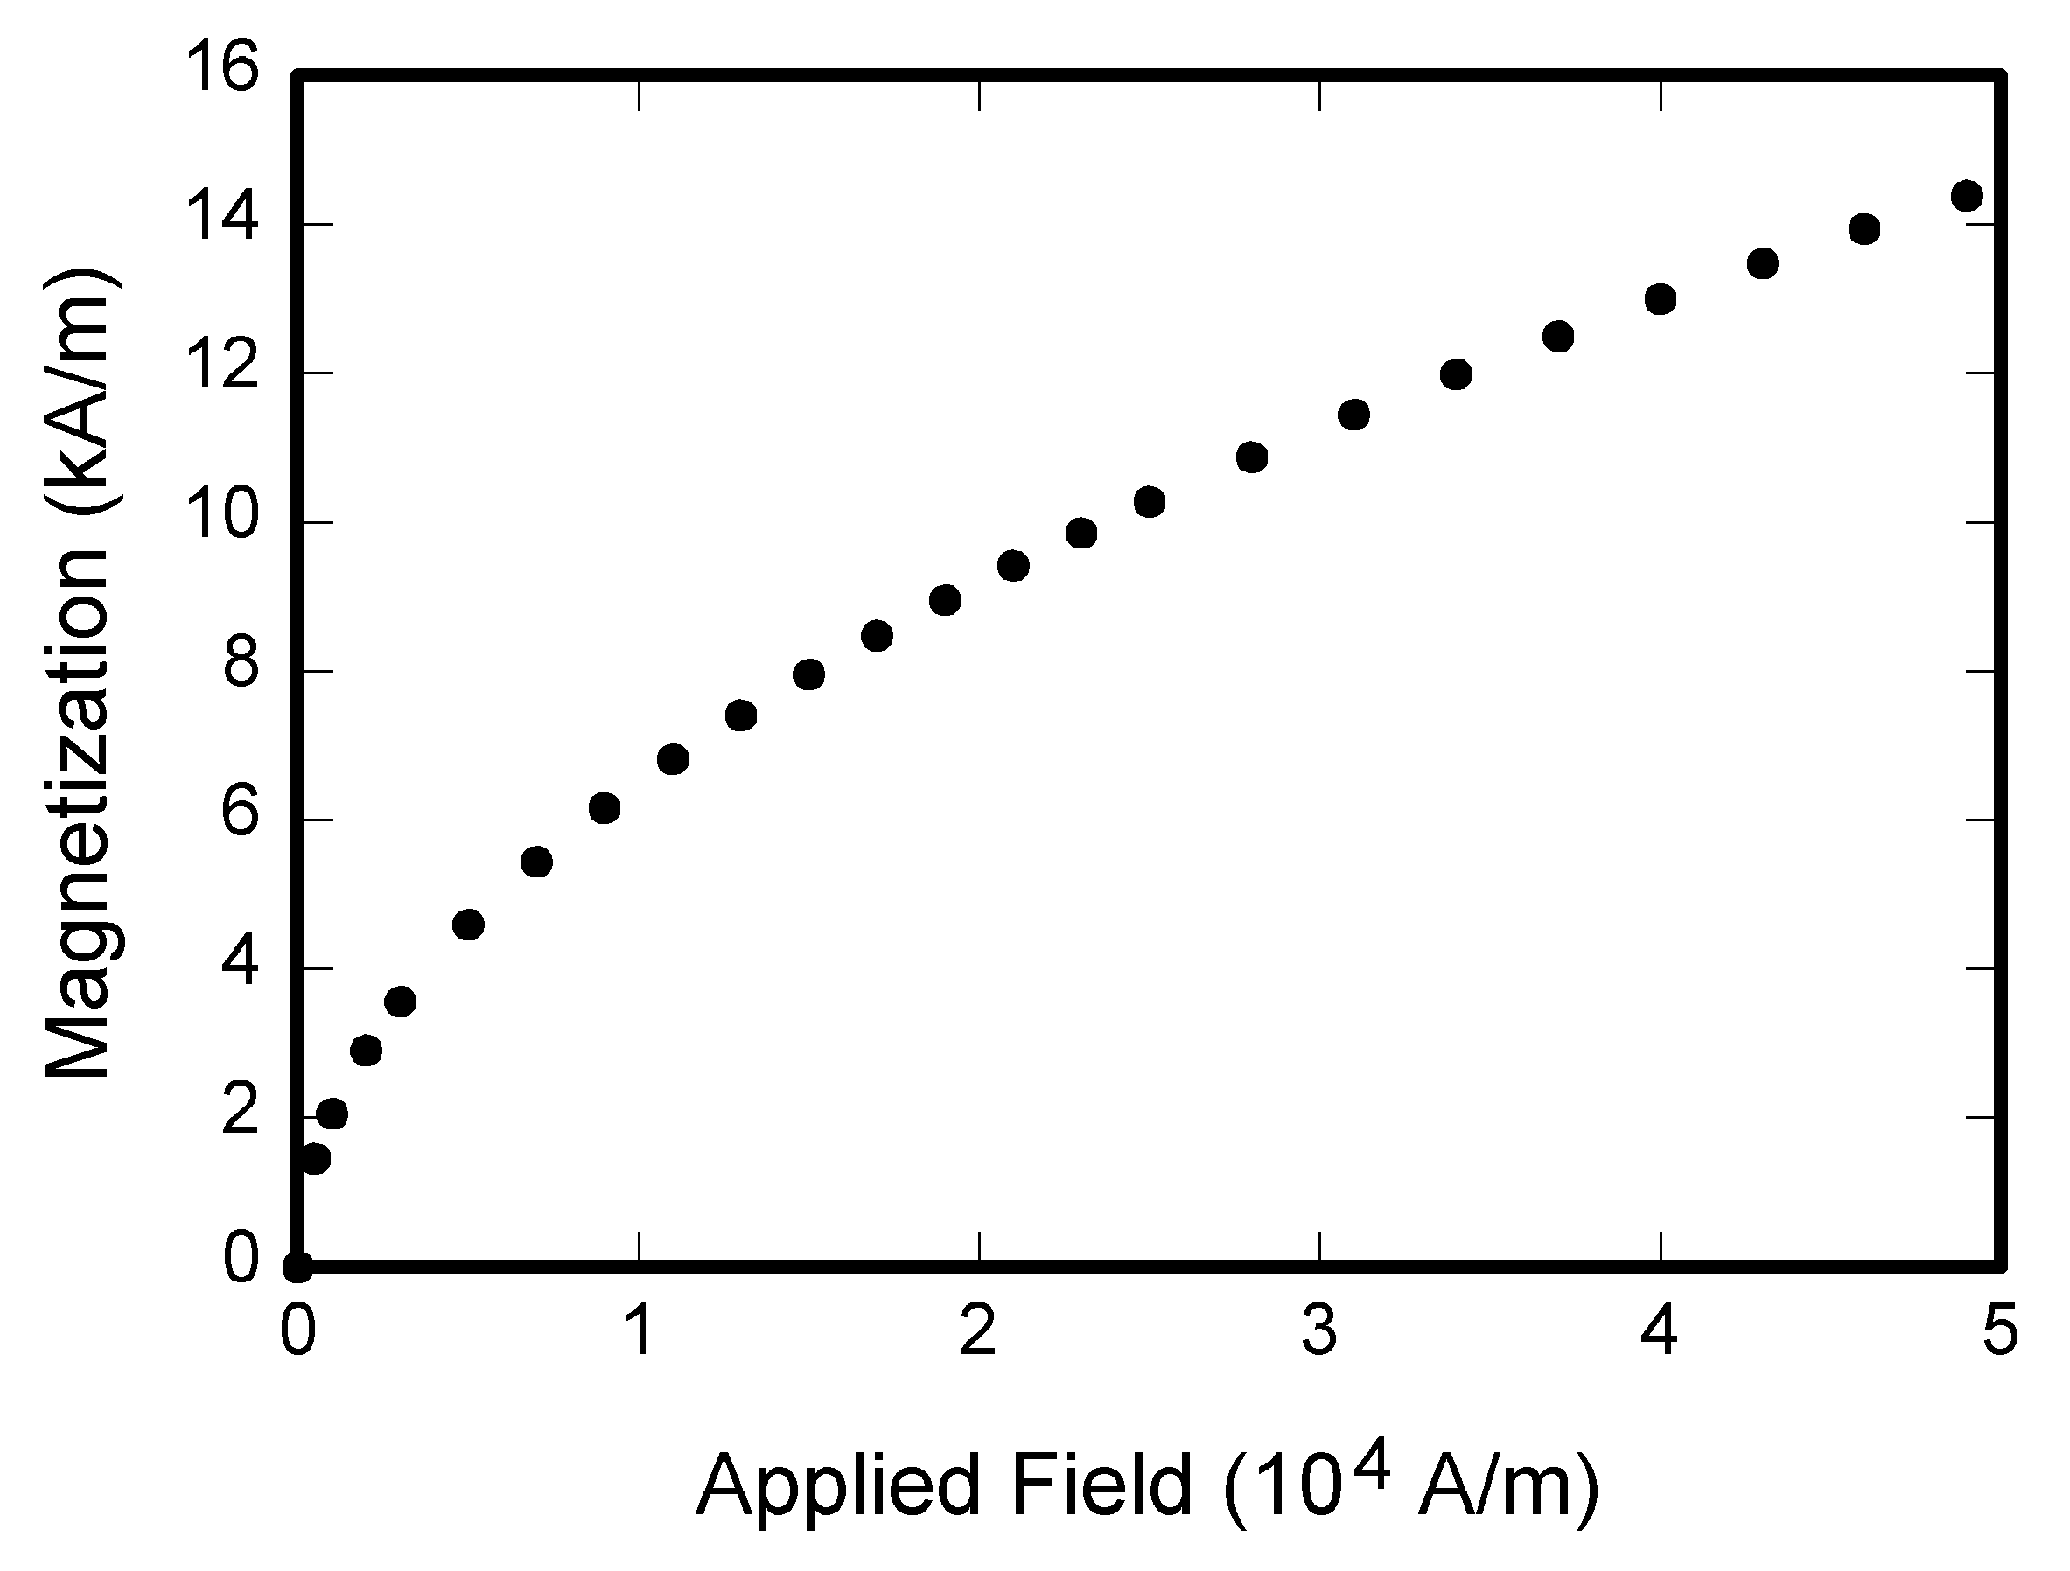
\includegraphics{fig1.png}}
\caption{Example of a figure caption.}
\label{fig}
\end{figure}

Figure Labels: Use 8 point Times New Roman for Figure labels. Use words 
rather than symbols or abbreviations when writing Figure axis labels to 
avoid confusing the reader. As an example, write the quantity 
``Magnetization'', or ``Magnetization, M'', not just ``M''. If including 
units in the label, present them within parentheses. Do not label axes only 
with units. In the example, write ``Magnetization (A/m)'' or ``Magnetization 
\{A[m(1)]\}'', not just ``A/m''. Do not label axes with a ratio of 
quantities and units. For example, write ``Temperature (K)'', not 
``Temperature/K''.

\section*{Acknowledgment}

The preferred spelling of the word ``acknowledgment'' in America is without 
an ``e'' after the ``g''. Avoid the stilted expression ``one of us (R. B. 
G.) thanks $\ldots$''. Instead, try ``R. B. G. thanks$\ldots$''. Put sponsor 
acknowledgments in the unnumbered footnote on the first page.

\begin{thebibliography}{00}
\bibitem{legion} Bauer, Michael, et al. "Legion: Expressing locality and independence with logical regions." SC'12: Proceedings of the International Conference on High Performance Computing, Networking, Storage and Analysis. IEEE, 2012.
\bibitem{charm} Kale, Laxmikant V., and Sanjeev Krishnan. "Charm++ a portable concurrent object oriented system based on c++." Proceedings of the eighth annual conference on Object-oriented programming systems, languages, and applications. 1993.
\bibitem{charm1} Kale, Laxmikant V., and Sanjeev Krishnan. "Charm++." (1996).
\bibitem{quark} AsimYarkhan.2012. DynamicTaskExecutiononSharedandDistributedMemory Architectures. December (2012). http://trace.tennessee.edu/utk
\bibitem{starpu} Augonnet, Cédric, Samuel Thibault, and Raymond Namyst. StarPU: a runtime system for scheduling tasks over accelerator-based multicore machines. Diss. INRIA, 2010.
\bibitem{halide} Ragan-Kelley, Jonathan, et al. "Halide: a language and compiler for optimizing parallelism, locality, and recomputation in image processing pipelines." Acm Sigplan Notices 48.6 (2013): 519-530.
\bibitem{dplasma} Bosilca, George, et al. "Flexible development of dense linear algebra algorithms on massively parallel architectures with DPLASMA." 2011 IEEE International Symposium on Parallel and Distributed Processing Workshops and Phd Forum. IEEE, 2011.
\bibitem{dague} Bosilca, George, et al. "DAGuE: A generic distributed DAG engine for high performance computing." Parallel Computing 38.1-2 (2012): 37-51.
\bibitem{regent} Slaughter, Elliott. Regent: A high-productivity programming language for implicit parallelism with logical regions. Diss. Stanford University, 2017.
\bibitem{regent1} Slaughter, Elliott, et al. "Regent: a high-productivity programming language for HPC with logical regions." Proceedings of the International Conference for High Performance Computing, Networking, Storage and Analysis. 2015.
\bibitem{luna} Belyaev, Nikolay, and Vladislav Perepelkin. "High-efficiency specialized support for dense linear algebra arithmetic in LuNA system." Parallel Computing Technologies: 16th International Conference, PaCT 2021, Kaliningrad, Russia, September 13–18, 2021, Proceedings 16. Springer International Publishing, 2021.
\bibitem{luna1} Belyaev, Nikolay, and Vladislav Perepelkin. "High-efficiency specialized support for dense linear algebra arithmetic in LuNA system." Parallel Computing Technologies: 16th International Conference, PaCT 2021, Kaliningrad, Russia, September 13–18, 2021, Proceedings 16. Springer International Publishing, 2021.
\end{thebibliography}

\vspace{12pt}
\color{red}
IEEE conference templates contain guidance text for composing and formatting conference papers. Please ensure that all template text is removed from your conference paper prior to submission to the conference. Failure to remove the template text from your paper may result in your paper not being published.

\end{document}
